\documentclass[xcolor={dvipsnames},aspectratio=169,10pt]{beamer}
% utility packages
\usepackage{etoolbox}
\usepackage{multicol}
\usepackage{relsize}
\usepackage{fontawesome}

% better text justifying
\usepackage{microtype}
% justify text inside list environment
% Ref: http://liam0205.me/2017/04/11/justifying-in-beamer-s-lists/
\usepackage{ragged2e}
\makeatletter
\patchcmd{\itemize}{\raggedright}{\justifying}{}{}
\patchcmd{\beamer@enum@}{\raggedright}{\justifying}{}{}
\patchcmd{\@@description}{\raggedright}{\justifying}{}{}
\makeatother

% math related packages
\usepackage{amsmath}
\usepackage[ruled,vlined]{algorithm2e}
\SetAlCapNameFnt{\scriptsize}
\SetAlCapFnt{\scriptsize}
\SetAlFnt{\scriptsize}

% figure related packages
\usepackage{graphicx}
\usepackage[scale=2]{ccicons}
\usepackage{qrcode}
\usepackage{tikz}
\usepackage{tikzpagenodes}
\usetikzlibrary{positioning}

% table related packages
\usepackage{array}
\usepackage{booktabs}
\usepackage{multirow}
\usepackage{colortbl}
\newcommand{\tabincell}[2]{\begin{tabular}{@{}#1@{}}#2\end{tabular}}

% code highlight
\usepackage{listings}
\usepackage{minted}
\definecolor{mintedbg}{HTML}{E5E9F0}
\setminted{autogobble,bgcolor=mintedbg,fontsize=\small}
\setmintedinline{bgcolor=mintedbg,fontsize=\smaller}
\newminted{bash}{}
\newminted{latex}{}
\newmintinline{bash}{}
\newmintinline{latex}{}
\newcommand{\texdoc}[2]{\href{#2}{\bashinline|texdoc #1|}}

% hyperref setting
\hypersetup{
  unicode,
  psdextra,
  bookmarksnumbered=true,
  bookmarksopen=true,
  bookmarksopenlevel=3,
  bookmarksdepth=4,
  pdfcenterwindow=true,
  pdfstartview={Fit},
  pdfpagemode={FullScreen},
  pdfpagelayout={SinglePage},
}
\usepackage{bookmark}

% beamer theme
\usetheme{metropolis}
\metroset{block=fill,numbering=fraction}

% caption style
\usepackage{subcaption}
\setlength\abovecaptionskip{3pt}
\setbeamerfont{caption}{size=\scriptsize}
\renewcommand{\figurename}{Fig.}
\captionsetup{labelformat=empty,labelsep=none,textfont={bf,it}}

% Ref: https://github.com/gpoore/minted/blob/master/source/minted.dtx
\newenvironment{latexexample}
{\VerbatimEnvironment\begin{VerbatimOut}[gobble=3]{example.out}}{\end{VerbatimOut}%
  \begin{center}
    \begin{minipage}{0.47\linewidth}%
      \inputminted[resetmargins,fontsize=\scriptsize]{latex}{example.out}%
    \end{minipage}%
    \hspace{0.05\linewidth}%
    \begin{minipage}{0.47\linewidth}%
      \begin{framed}
        \setlength{\parindent}{2em}%
        \input{example.out}%
      \end{framed}
    \end{minipage}%
  \end{center}
}

\newenvironment{mathexample}
{\VerbatimEnvironment\begin{VerbatimOut}[gobble=3]{example.out}}{\end{VerbatimOut}%
  \begin{center}
    \begin{minipage}{0.47\linewidth}%
      \inputminted[resetmargins,fontsize=\scriptsize]{latex}{example.out}%
    \end{minipage}%
    \hspace{0.05\linewidth}%
    \begin{minipage}{0.47\linewidth}%
      \begin{framed}
        \[ \input{example.out} \]
      \end{framed}
    \end{minipage}%
  \end{center}
}

\newenvironment{mathexamples}
{\VerbatimEnvironment\begin{VerbatimOut}[gobble=3]{example.out}}{\end{VerbatimOut}%
  \begin{center}
    \begin{minipage}{0.47\linewidth}%
      \inputminted[resetmargins,fontsize=\scriptsize]{latex}{example.out}%
    \end{minipage}%
    \hspace{0.05\linewidth}%
    \begin{minipage}{0.47\linewidth}%
      \begin{framed}
        \directlua{
          local first = true
          for line in io.lines('example.out') do
          if first then
          first = false
          else
          tex.print('\\newline ')
          end
          tex.print('$' .. line .. '$')
          end
        }
      \end{framed}
    \end{minipage}%
  \end{center}
}


\title{The Future of Engineering}
\subtitle{Challenges and opportunities }
\author{Miguel Xochicale  (\faGithub @mxochicale  \faTwitter @\_mxochicale) 
}
\date{October 21, 2020; 18h00m MEX\\
	  Conf of Eng and Tech for Suistanable Development}
\institute{
	School of Biomedical Engineering and Imaging Sciences \\
	King's College London
	}

\titlegraphic{
  \begin{tikzpicture}[overlay, remember picture]
    \node[%
      above right=0.35cm and -0.2cm of current page footer area.south west,
      anchor=south west,
      inner sep=0pt] {%
      \usebeamerfont{footline}
      \begin{tabular}{lm{.8\textwidth}}
        \href{http://creativecommons.org/licenses/by/4.0/}{\ccby} &
        This work is licensed under a 
	\href{http://creativecommons.org/licenses/by/4.0/}
		{Creative Commons ``Attribution 4.0 International''} license. 
	\par Get source of this slides and see further references 
		from \url{https://github.com/mxochicale/itds2020}.
      \end{tabular}
    };
    \node[%
      above left=0.35cm and 0cm of current page footer area.south east,
      anchor=south east,
      inner sep=0pt]{\qrcode[height=1.5cm]{https://github.com/mxochicale/}};
  \end{tikzpicture}
}

\begin{document}

\maketitle

\begin{frame}{Contents}
    \tableofcontents
\end{frame}

%%%%%%%%%%%%%%%%%%%%%%%%%%%%%%%%%%%%%%%%%%%%
\section{Short-bio}

\begin{frame}{My journey in science}

\begin{itemize}	
	\item \textbf{(1996-1999)} High School in Electronics
	\item \textbf{(1999-2004)} BSc in Electronics  
	\item \textbf{(2004-2006)} MSc in Signal Processing 
	\item \textbf{(2006-2012)} Teaching Associate in Mechatronics 
	\item \textbf{(2013-2014)} Research Assistant in Robotics at INAOE  
	\item \textbf{(2014-2019)} PhD student in Human-Robot Interaction at Uni of Bham \\
	\item \textbf{(2019-present)} Research Associate in Ultrasound-Guidance 
	Intervention at KCL 
\end{itemize}

	\vspace{4mm}
        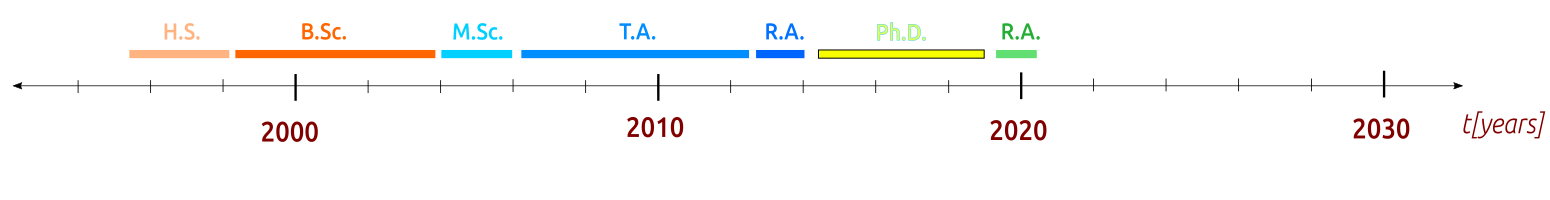
\includegraphics[width=\linewidth]{./figs/myjourney/versions/drawing.png}

\end{frame}






%%%%%%%%%%%%%%%%%%%%%%%%%%%%%%%%%%%%%%%%%%%%
\section{Challenges and Opportunities in Engineering}

{
\paper{engineeringchallenges.org/challenges.aspx}
\begin{frame}{Challenges in Engineering}
  \begin{columns}
    \begin{column}{.6\linewidth}
    \begin{itemize}
    \item \textbf{Advance Personalised learning}
    \item \textbf{Make Solar Energy Economical}
    \item \textbf{Enhance Virtual Reality}
    \item \textbf{Reverse-engineer the brain}
    \item \textbf{Egineer better medicines}
    \item \textbf{Advance Health Informatics}
    \item \textbf{Restore and improve urban infrastructure}
    \item \textbf{Secure cyberspace}
    \item \textbf{Provide access to clean water}
    \item \textbf{Provide energy from fusion}
    \item \textbf{Develop Carbon Sequestration Methods}
    \item \textbf{Engineer the tools for science discovery}
    \end{itemize}
  \end{column}

  \begin{column}{.4\linewidth}
      \begin{figure}
        \centering
        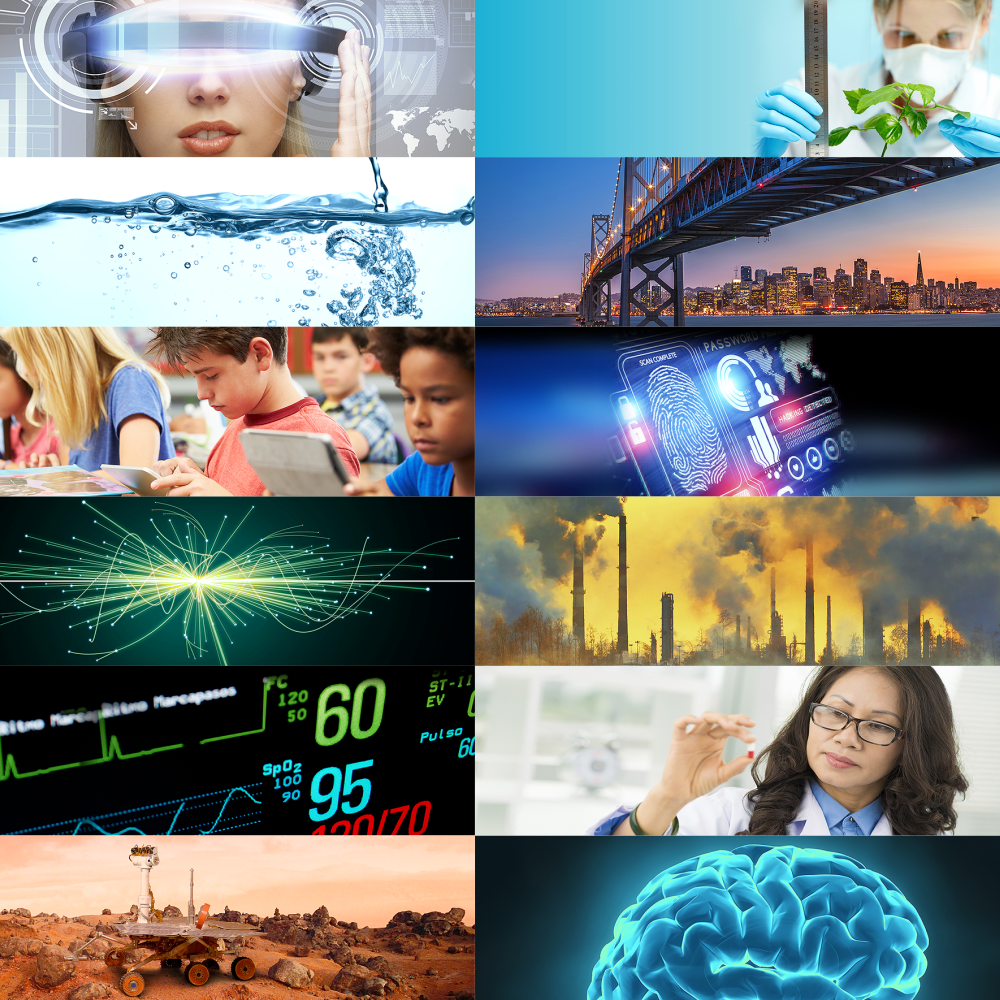
\includegraphics[scale=0.2]{./figs/challenges/versions/drawing-v01.png}
        \caption{}
      \end{figure}
    \end{column}
  \end{columns}

\end{frame}
}






%%%%%%%%%%%%%%%%%%%%%%%%%%%%%%%%%%%%%%%%%%%%
\subsection{Engineering as Multidisciplinary Field}

{
\paper{\textbf{Khanna and Kumar 2020} in Engineering 4.0: Future with Disruptive Technologies, DOI:10.1007/978-981-15-1137-07}
\begin{frame}{Engineering as Multidisciplinary Field}
    \begin{figure}
        \centering
        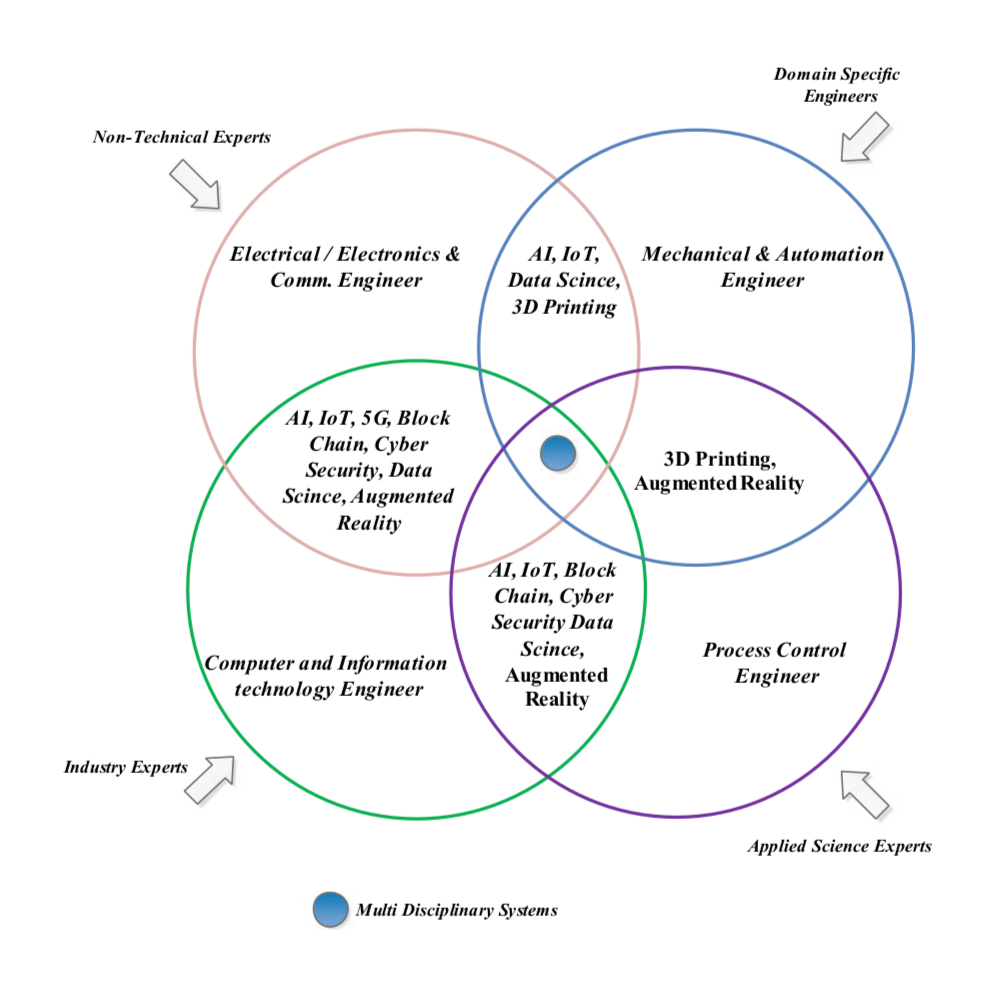
\includegraphics[width=0.55\linewidth]{./figs/multidisciplinary-engigneering/versions/drawing-v00.png}
        \caption{}
    \end{figure}
\end{frame}
}


%%%%%%%%%%%%%%%%%%%%%%%%%%%%%%%%%%%%%%%%%%%%
\subsection{Mechatronics and Robotics Engineering}
\begin{frame}{Robotics Engineering }
    \begin{figure}
        \centering
        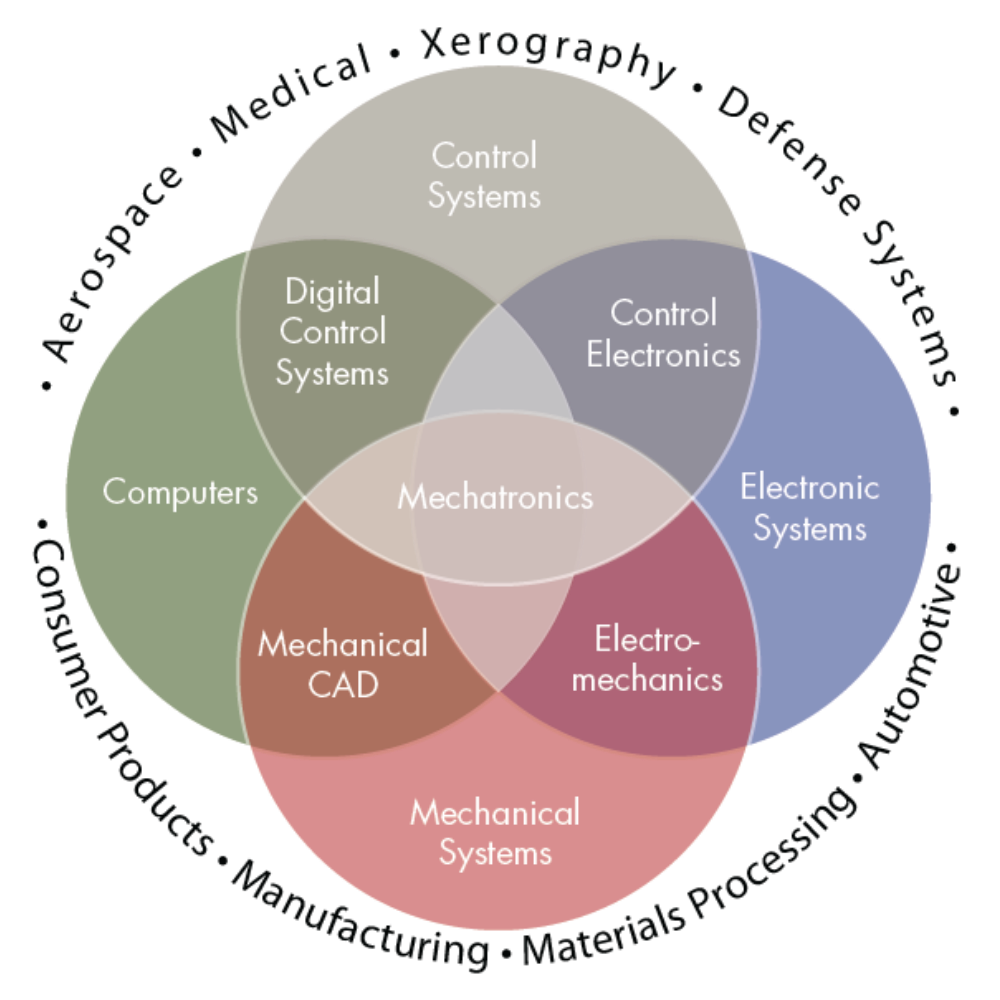
\includegraphics[width=0.5\linewidth]{./figs/robotics/versions/drawing.png}
        \caption{}
    \end{figure}
\end{frame}


%%%%%%%%%%%%%%%%%%%%%%%%%%%%%%%%%%%%%%%%%%%%
\subsection{Open-source projects}
{
%\paper{\textbf{Xochicale 2020} in Conf. of Reproducibility, Replicability and Trust in Science \faGithub github.com/mxochicale/rrts2020}
\begin{frame}{Open-source projects}
    \vspace{-00mm}
      \begin{figure}
        \centering
        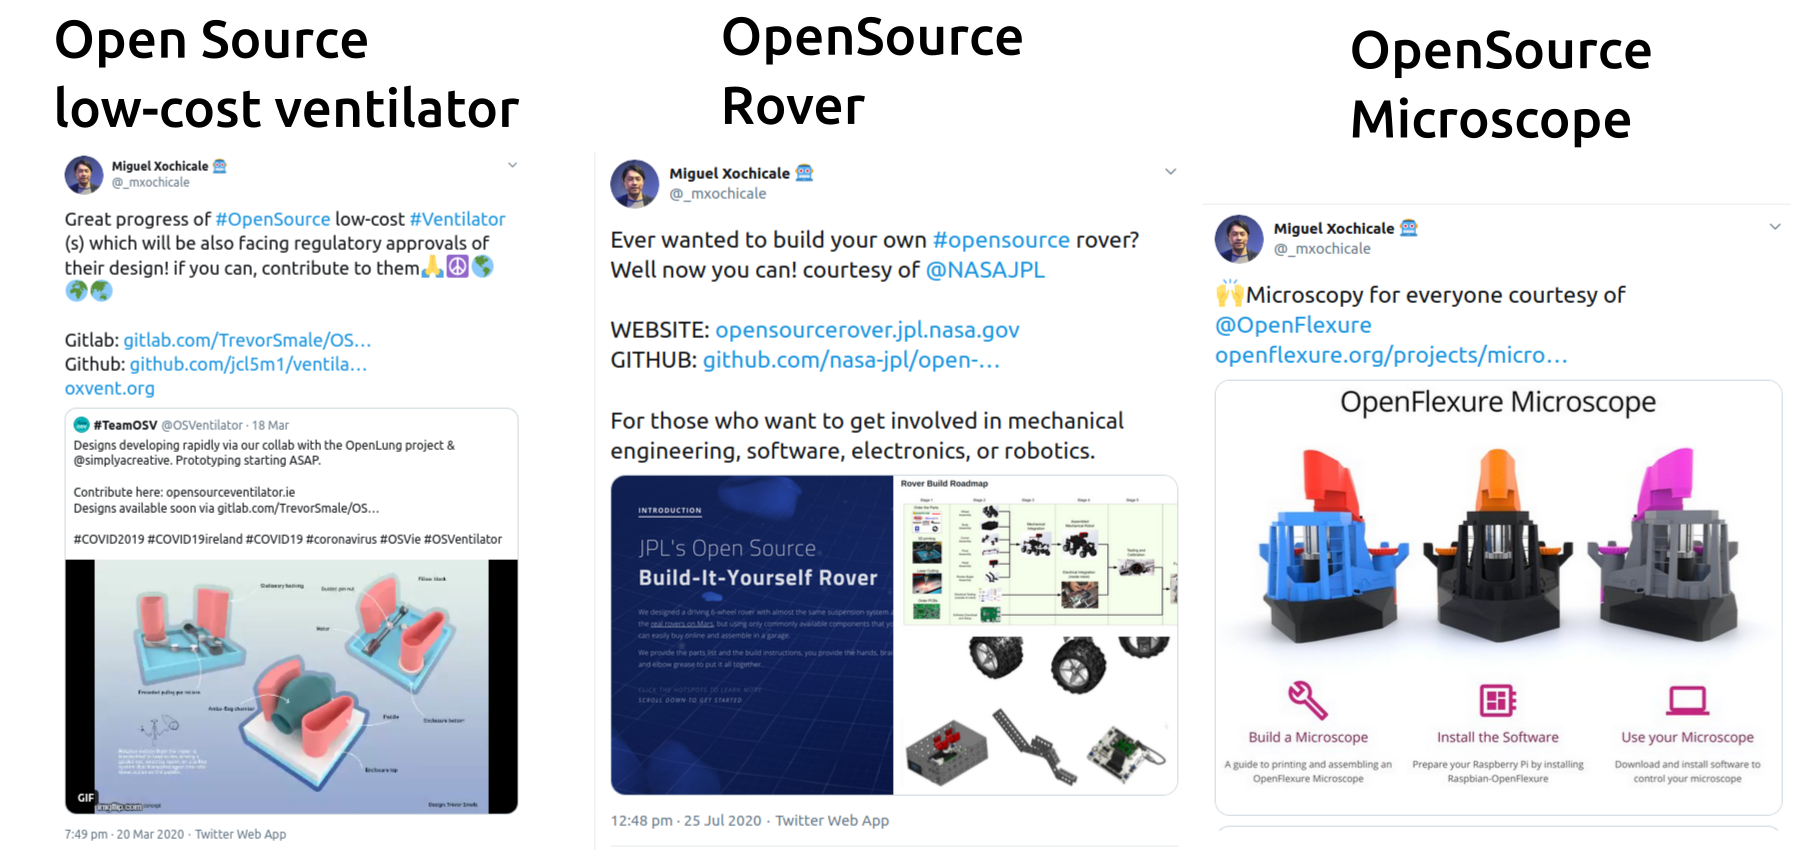
\includegraphics[width=\linewidth]{./figs/oa-projects/versions/drawing-v00.png}
        \caption{}
      \end{figure}
\end{frame}
}



%%%%%%%%%%%%%%%%%%%%%%%%%%%%%%%%%%%%%%%%%%%%
\section{The Future Engineering }

{
\paper{\textbf{Xochicale 2020} in Conf. of Reproducibility, Replicability and Trust in Science \faGithub github.com/mxochicale/rrts2020}
\begin{frame}{Introduction}
      \begin{figure}
        \centering
        %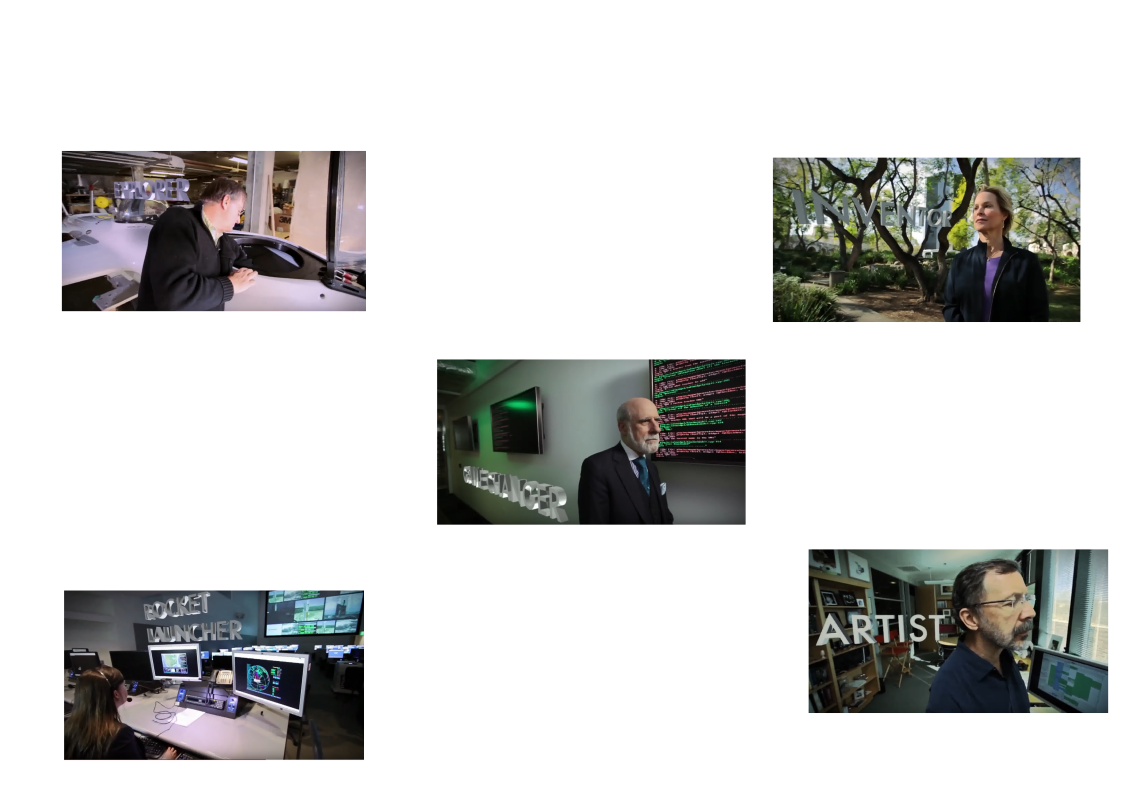
\includegraphics[width=\linewidth]{./figs/eng-of-the-future/versions/drawing.png}
        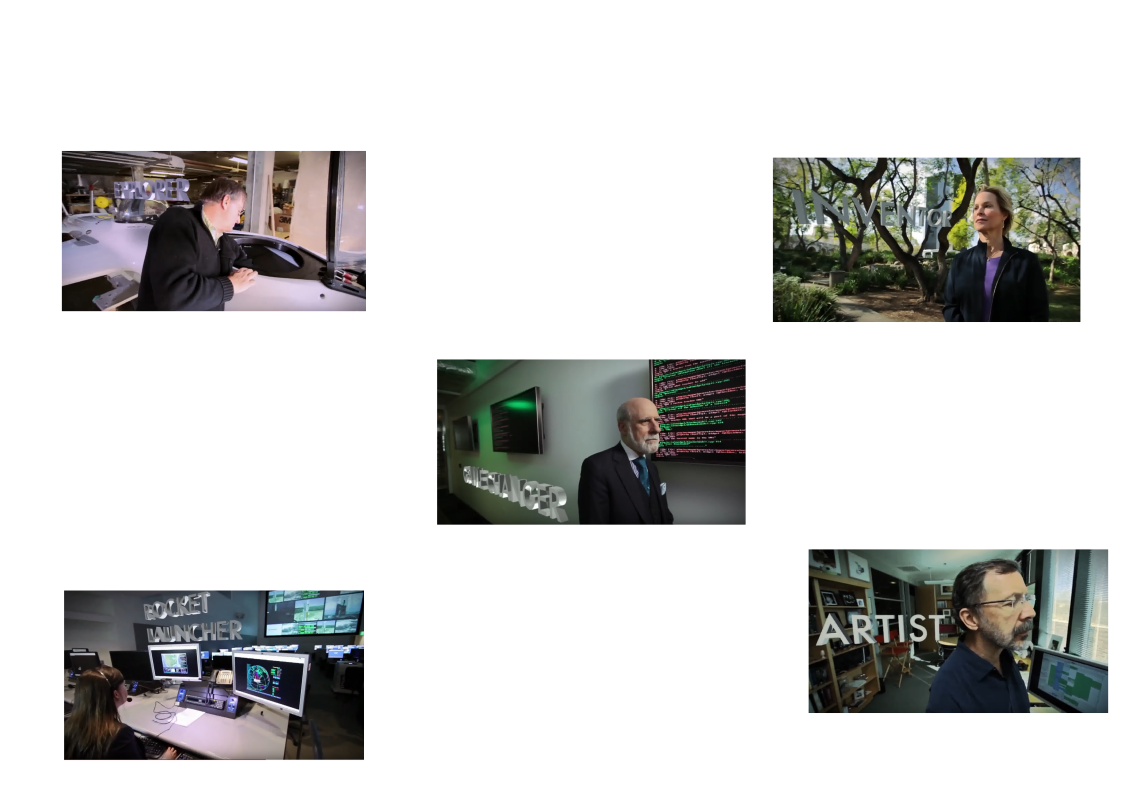
\includegraphics[scale=0.2]{./figs/eng-of-the-future/versions/drawing.png}
        \caption{Compile \LaTeX~Project in VSCode}
      \end{figure}

\end{frame}
}


\begin{frame}{Introduction}
  \begin{itemize}
    \item \alert{\LaTeX{}} is a document preparation system and document markup language.
    \item It can be used to typeset articles, books, slides, posters, even graphics.
    \item \textbf{\textcolor{Green}{Pros}:}
          \begin{itemize}
            \item It separates presentation/format from contents.
            \item Since the source codes are plaintext, it works well with version control system such as git.
            \item Highly customizable through various of packages.
          \end{itemize}
    \item \textbf{\textcolor{Red}{Cons}:}
          \begin{itemize}
            \item There is no graphic interface to support WYSIWYG style editing.
            \item Not suitable to produce unstructured documents.
          \end{itemize}
  \end{itemize}
\end{frame}




%%%%%%%%%%%%%%%%%%%%%%%%%%%%%%%%%%%%%%%%%%%%
\section{My lines of research}
{
\paper{\textbf{M. Xochicale 2019} PhD thesis, DOI:10.5281/zenodo.3384145}
\begin{frame}{Variabilty in HRI using nonlinear dynamics}
    \vspace{-00mm}
      \begin{figure}
        \centering
        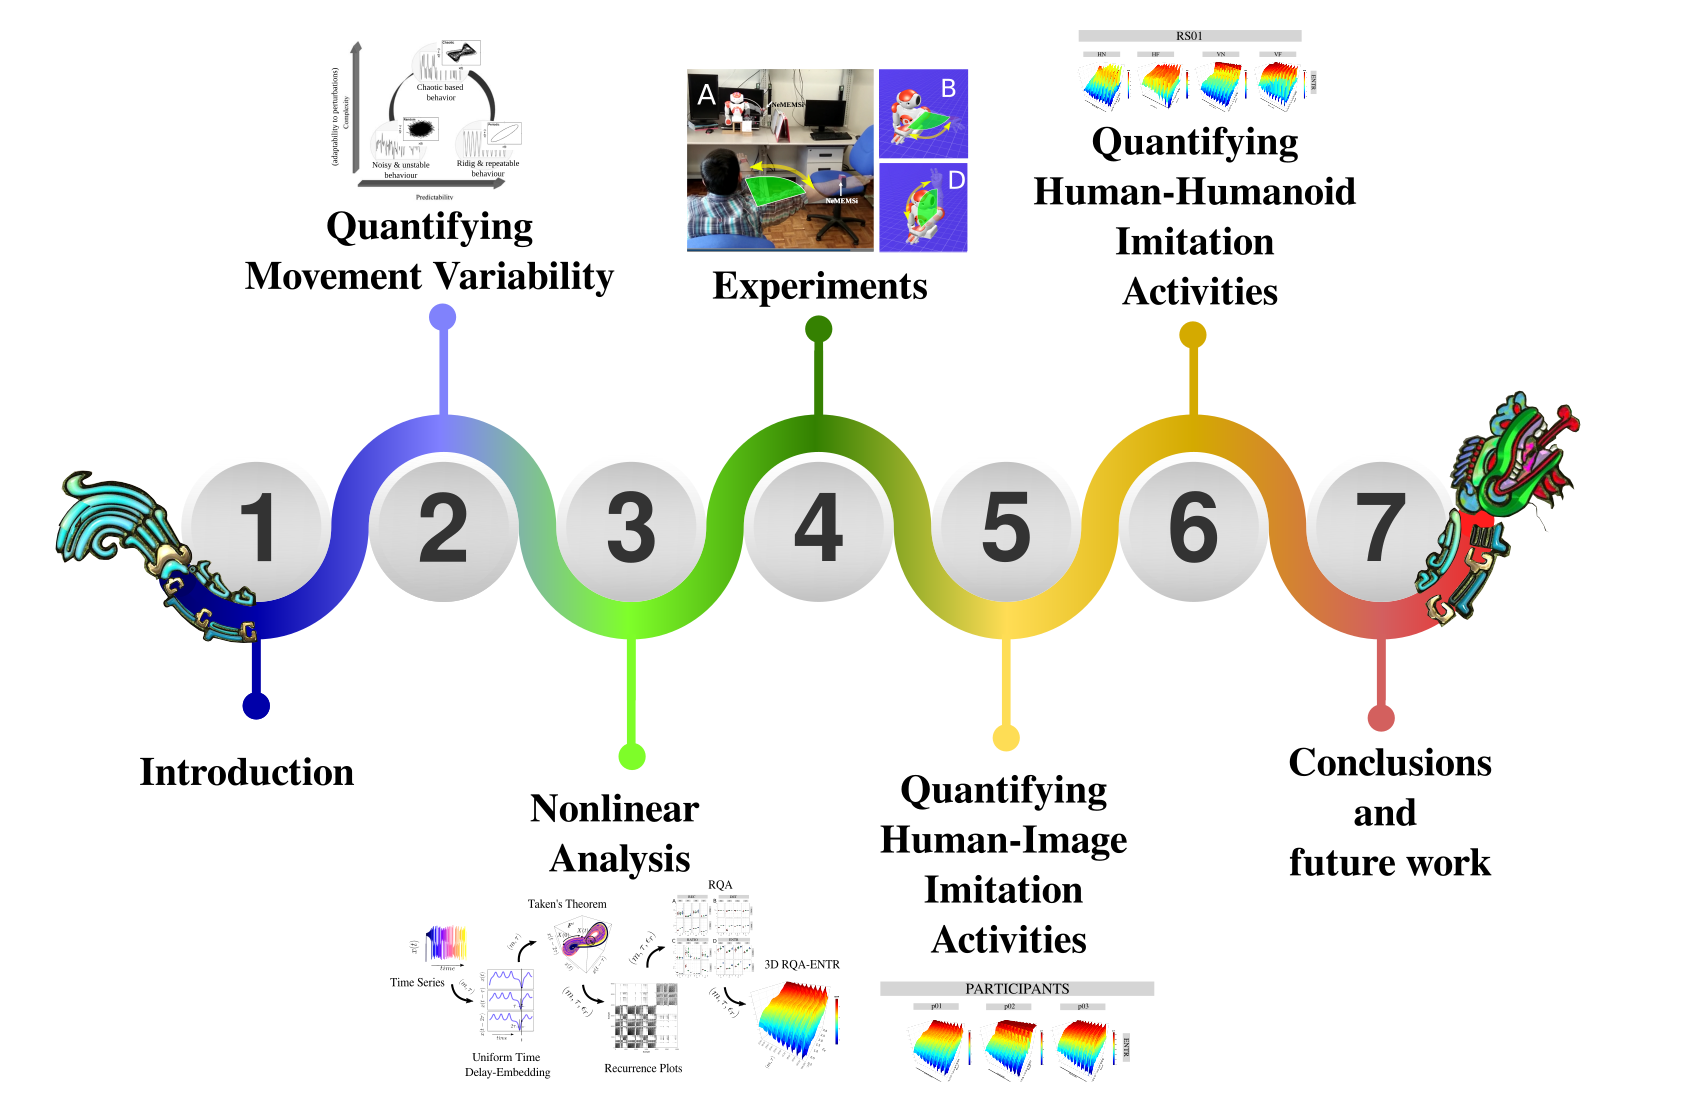
\includegraphics[width=0.8\linewidth]{./figs/oa-thesis/versions/drawing-v00.png}
        \caption{}
      \end{figure}
\end{frame}
}

{
\paper{\textbf{M. Xochicale 2019} GITHUB: https://github.com/air4children}
\begin{frame}{Artificial Intelligence and Robotics for Children}
    \vspace{-00mm}
      \begin{figure}
        \centering
        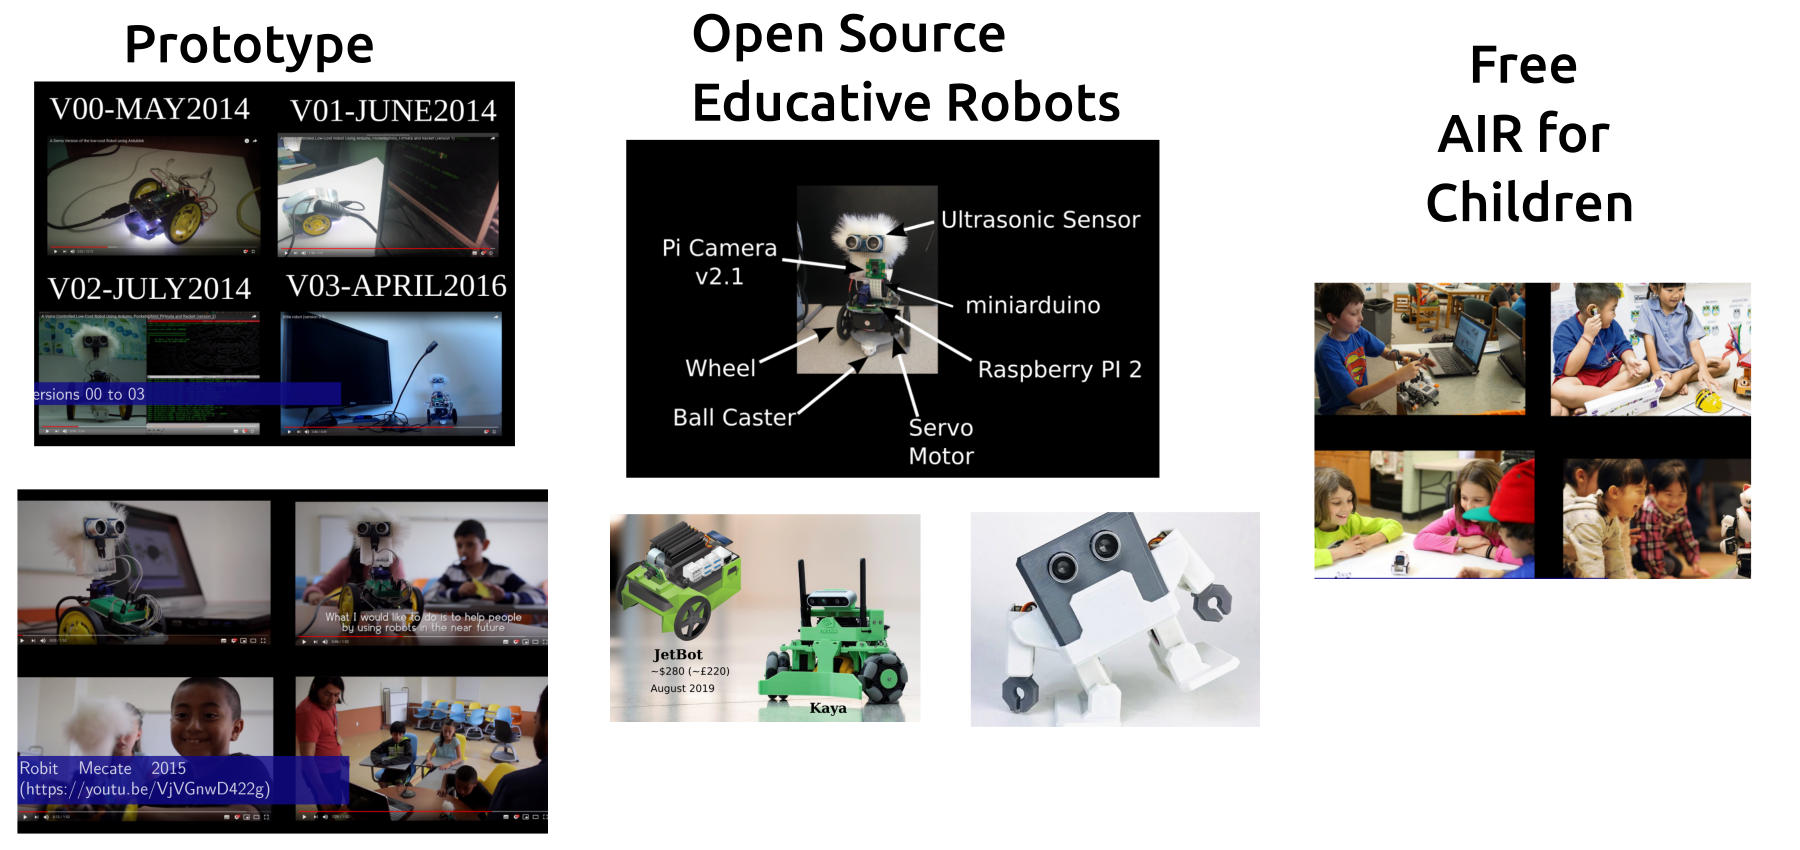
\includegraphics[width=0.8\linewidth]{./figs/air4children/versions/drawing-v00.png}
        \caption{}
      \end{figure}
\end{frame}
}




\begin{frame}[standout]
  Thanks \\
  Questions?
\end{frame}

\end{document}
